% Options for packages loaded elsewhere
\PassOptionsToPackage{unicode}{hyperref}
\PassOptionsToPackage{hyphens}{url}
%
\documentclass[
]{article}
\usepackage{lmodern}
\usepackage{amssymb,amsmath}
\usepackage{ifxetex,ifluatex}
\ifnum 0\ifxetex 1\fi\ifluatex 1\fi=0 % if pdftex
  \usepackage[T1]{fontenc}
  \usepackage[utf8]{inputenc}
  \usepackage{textcomp} % provide euro and other symbols
\else % if luatex or xetex
  \usepackage{unicode-math}
  \defaultfontfeatures{Scale=MatchLowercase}
  \defaultfontfeatures[\rmfamily]{Ligatures=TeX,Scale=1}
\fi
% Use upquote if available, for straight quotes in verbatim environments
\IfFileExists{upquote.sty}{\usepackage{upquote}}{}
\IfFileExists{microtype.sty}{% use microtype if available
  \usepackage[]{microtype}
  \UseMicrotypeSet[protrusion]{basicmath} % disable protrusion for tt fonts
}{}
\makeatletter
\@ifundefined{KOMAClassName}{% if non-KOMA class
  \IfFileExists{parskip.sty}{%
    \usepackage{parskip}
  }{% else
    \setlength{\parindent}{0pt}
    \setlength{\parskip}{6pt plus 2pt minus 1pt}}
}{% if KOMA class
  \KOMAoptions{parskip=half}}
\makeatother
\usepackage{xcolor}
\IfFileExists{xurl.sty}{\usepackage{xurl}}{} % add URL line breaks if available
\IfFileExists{bookmark.sty}{\usepackage{bookmark}}{\usepackage{hyperref}}
\hypersetup{
  pdftitle={TS simulations - ZooScatR},
  pdfauthor={Sven Gastauer},
  hidelinks,
  pdfcreator={LaTeX via pandoc}}
\urlstyle{same} % disable monospaced font for URLs
\usepackage[margin=1in]{geometry}
\usepackage{color}
\usepackage{fancyvrb}
\newcommand{\VerbBar}{|}
\newcommand{\VERB}{\Verb[commandchars=\\\{\}]}
\DefineVerbatimEnvironment{Highlighting}{Verbatim}{commandchars=\\\{\}}
% Add ',fontsize=\small' for more characters per line
\usepackage{framed}
\definecolor{shadecolor}{RGB}{248,248,248}
\newenvironment{Shaded}{\begin{snugshade}}{\end{snugshade}}
\newcommand{\AlertTok}[1]{\textcolor[rgb]{0.94,0.16,0.16}{#1}}
\newcommand{\AnnotationTok}[1]{\textcolor[rgb]{0.56,0.35,0.01}{\textbf{\textit{#1}}}}
\newcommand{\AttributeTok}[1]{\textcolor[rgb]{0.77,0.63,0.00}{#1}}
\newcommand{\BaseNTok}[1]{\textcolor[rgb]{0.00,0.00,0.81}{#1}}
\newcommand{\BuiltInTok}[1]{#1}
\newcommand{\CharTok}[1]{\textcolor[rgb]{0.31,0.60,0.02}{#1}}
\newcommand{\CommentTok}[1]{\textcolor[rgb]{0.56,0.35,0.01}{\textit{#1}}}
\newcommand{\CommentVarTok}[1]{\textcolor[rgb]{0.56,0.35,0.01}{\textbf{\textit{#1}}}}
\newcommand{\ConstantTok}[1]{\textcolor[rgb]{0.00,0.00,0.00}{#1}}
\newcommand{\ControlFlowTok}[1]{\textcolor[rgb]{0.13,0.29,0.53}{\textbf{#1}}}
\newcommand{\DataTypeTok}[1]{\textcolor[rgb]{0.13,0.29,0.53}{#1}}
\newcommand{\DecValTok}[1]{\textcolor[rgb]{0.00,0.00,0.81}{#1}}
\newcommand{\DocumentationTok}[1]{\textcolor[rgb]{0.56,0.35,0.01}{\textbf{\textit{#1}}}}
\newcommand{\ErrorTok}[1]{\textcolor[rgb]{0.64,0.00,0.00}{\textbf{#1}}}
\newcommand{\ExtensionTok}[1]{#1}
\newcommand{\FloatTok}[1]{\textcolor[rgb]{0.00,0.00,0.81}{#1}}
\newcommand{\FunctionTok}[1]{\textcolor[rgb]{0.00,0.00,0.00}{#1}}
\newcommand{\ImportTok}[1]{#1}
\newcommand{\InformationTok}[1]{\textcolor[rgb]{0.56,0.35,0.01}{\textbf{\textit{#1}}}}
\newcommand{\KeywordTok}[1]{\textcolor[rgb]{0.13,0.29,0.53}{\textbf{#1}}}
\newcommand{\NormalTok}[1]{#1}
\newcommand{\OperatorTok}[1]{\textcolor[rgb]{0.81,0.36,0.00}{\textbf{#1}}}
\newcommand{\OtherTok}[1]{\textcolor[rgb]{0.56,0.35,0.01}{#1}}
\newcommand{\PreprocessorTok}[1]{\textcolor[rgb]{0.56,0.35,0.01}{\textit{#1}}}
\newcommand{\RegionMarkerTok}[1]{#1}
\newcommand{\SpecialCharTok}[1]{\textcolor[rgb]{0.00,0.00,0.00}{#1}}
\newcommand{\SpecialStringTok}[1]{\textcolor[rgb]{0.31,0.60,0.02}{#1}}
\newcommand{\StringTok}[1]{\textcolor[rgb]{0.31,0.60,0.02}{#1}}
\newcommand{\VariableTok}[1]{\textcolor[rgb]{0.00,0.00,0.00}{#1}}
\newcommand{\VerbatimStringTok}[1]{\textcolor[rgb]{0.31,0.60,0.02}{#1}}
\newcommand{\WarningTok}[1]{\textcolor[rgb]{0.56,0.35,0.01}{\textbf{\textit{#1}}}}
\usepackage{graphicx,grffile}
\makeatletter
\def\maxwidth{\ifdim\Gin@nat@width>\linewidth\linewidth\else\Gin@nat@width\fi}
\def\maxheight{\ifdim\Gin@nat@height>\textheight\textheight\else\Gin@nat@height\fi}
\makeatother
% Scale images if necessary, so that they will not overflow the page
% margins by default, and it is still possible to overwrite the defaults
% using explicit options in \includegraphics[width, height, ...]{}
\setkeys{Gin}{width=\maxwidth,height=\maxheight,keepaspectratio}
% Set default figure placement to htbp
\makeatletter
\def\fps@figure{htbp}
\makeatother
\setlength{\emergencystretch}{3em} % prevent overfull lines
\providecommand{\tightlist}{%
  \setlength{\itemsep}{0pt}\setlength{\parskip}{0pt}}
\setcounter{secnumdepth}{-\maxdimen} % remove section numbering
\usepackage{booktabs}
\usepackage{longtable}
\usepackage{array}
\usepackage{multirow}
\usepackage{wrapfig}
\usepackage{float}
\usepackage{colortbl}
\usepackage{pdflscape}
\usepackage{tabu}
\usepackage{threeparttable}
\usepackage{threeparttablex}
\usepackage[normalem]{ulem}
\usepackage{makecell}

\title{TS simulations - ZooScatR}
\author{Sven Gastauer}
\date{10/09/2020}

\begin{document}
\maketitle

\begin{Shaded}
\begin{Highlighting}[]
\CommentTok{#tidyverse for cleaner code}
\KeywordTok{library}\NormalTok{(tidyr)}
\KeywordTok{library}\NormalTok{(dplyr)}
\KeywordTok{library}\NormalTok{(purrr)}
\CommentTok{#apply with progress}
\KeywordTok{library}\NormalTok{(pbapply)}

\CommentTok{#plotting}
\KeywordTok{library}\NormalTok{(ggplot2)}

\CommentTok{#special libraries}
\KeywordTok{library}\NormalTok{(ZooScatR)}

\CommentTok{#pdf stuff}
\KeywordTok{library}\NormalTok{(kableExtra)}
\KeywordTok{library}\NormalTok{(knitr)}

\CommentTok{#define if simulations should be multithreadded. THis will run the simulations in parallel using with # cores avaialbale -1}
\NormalTok{runParallel =}\StringTok{ }\OtherTok{TRUE}
\ControlFlowTok{if}\NormalTok{ (runParallel }\OperatorTok{==}\StringTok{ }\OtherTok{TRUE}\NormalTok{)\{}
  \KeywordTok{library}\NormalTok{(foreach)}
  \KeywordTok{library}\NormalTok{(doParallel)}
  
  \KeywordTok{registerDoParallel}\NormalTok{(parallel}\OperatorTok{::}\KeywordTok{detectCores}\NormalTok{()}\OperatorTok{-}\DecValTok{1}\NormalTok{)}
\NormalTok{\}}
\CommentTok{#force running a new simulation, even if an RDS file with simualtions is available}
\NormalTok{force=}\OtherTok{TRUE}
\CommentTok{#set working dir}
\KeywordTok{setwd}\NormalTok{(}\StringTok{'C:}\CharTok{\textbackslash{}\textbackslash{}}\StringTok{Users}\CharTok{\textbackslash{}\textbackslash{}}\StringTok{mbd}\CharTok{\textbackslash{}\textbackslash{}}\StringTok{phd}\CharTok{\textbackslash{}\textbackslash{}}\StringTok{ZooScatStuff}\CharTok{\textbackslash{}\textbackslash{}}\StringTok{'}\NormalTok{)}
\end{Highlighting}
\end{Shaded}

\hypertarget{a-priori-assumptions}{%
\subsection{A priori assumptions}\label{a-priori-assumptions}}

We assume copepods, euphausiids, appendicularians and chaetognaths to be
the dominant species groups. For diverse Calanus groups, cheatognaths
and euphausiids, we can use literature values to populate the model. I
couldn't find any values for appendicularians, so I used values for fish
larvae here as an approximation.

\hypertarget{model-definition}{%
\subsection{Model definition}\label{model-definition}}

Let's start by loading some standard values for the model:

\begin{Shaded}
\begin{Highlighting}[]
\CommentTok{#number of simulations}
\NormalTok{nsim =}\StringTok{ }\DecValTok{100}
\CommentTok{#location of the standard parameter file contained within the package}
\NormalTok{fname <-}\StringTok{ }\KeywordTok{paste0}\NormalTok{(}\KeywordTok{system.file}\NormalTok{(}\DataTypeTok{package=}\StringTok{"ZooScatR"}\NormalTok{),}\StringTok{"/extdata/configs/config_0.dat"}\NormalTok{)}
\CommentTok{# read the parameters file}
\NormalTok{para =}\StringTok{ }\NormalTok{ZooScatR}\OperatorTok{::}\KeywordTok{read_para}\NormalTok{(fname)}
\CommentTok{#set the soundspeed in the surrounding sea water}
\NormalTok{misc <-}\StringTok{ }\KeywordTok{list}\NormalTok{(}\DataTypeTok{cw=}\DecValTok{1500}\NormalTok{)}
\CommentTok{#let's set the start and end frequencies}
\NormalTok{f0=}\DecValTok{200} \CommentTok{#eill bepara$simu$var0}
\NormalTok{f1=}\DecValTok{1000} \CommentTok{#will be para$simu$var1}
\CommentTok{#number of output frequencies}
\NormalTok{nf=}\DecValTok{801} \CommentTok{#will be para$simu$n}
\end{Highlighting}
\end{Shaded}

For the parameter distributions a gamma, normal or uniform dsitribution
were used.\\
For gamma distributions a density function with a shape \(s\) and a rate
\(a\) was defined as:

\[f_{\Gamma}(x)= \frac{1}{s^a \Gamma(a) x^{a-1} e^{-\frac{x}{s}}}\]
where \(\Gamma(a)\) is defined as
{[}@milne-thomson\_handbook\_1972{]}:\\
\[\Gamma(a)=\int_0^\infty{t^{a-1}e^{-t} dt}\]

Normal distributions were computed with standard deviation \(\sigma\)
and mean \(\mu\) with a density given by
{[}@johnson\_continuous\_1995{]}:
\[f_N(x)=\frac{1}{\sqrt{2\pi}\sigma e^{-{\frac{(x-\mu)^2}{2\sigma^2}}}}\]
A summary of the settings is defined in table 1.

For euphausiids a bimodal truncated normal distribution was used.

\begin{Shaded}
\begin{Highlighting}[]
\NormalTok{pm =}\StringTok{ }\KeywordTok{data.frame}\NormalTok{(}\DataTypeTok{species=}\KeywordTok{c}\NormalTok{(}\StringTok{'copepod'}\NormalTok{,}\StringTok{'Euphausiids1'}\NormalTok{,}\StringTok{'Euphausiids2'}\NormalTok{,}\StringTok{'Chaetognaths'}\NormalTok{,}\StringTok{'Appendicularians'}\NormalTok{),}
  \DataTypeTok{L_dist=}\KeywordTok{c}\NormalTok{(}\StringTok{'gamma'}\NormalTok{, }\StringTok{'truncated normal'}\NormalTok{,}\StringTok{'truncated normal'}\NormalTok{, }\StringTok{'gamma'}\NormalTok{,}\StringTok{'gamma'}\NormalTok{),}
  \DataTypeTok{L_shape=}\KeywordTok{c}\NormalTok{(}\DecValTok{7}\NormalTok{, }\DecValTok{3}\NormalTok{,}\DecValTok{20}\NormalTok{, }\DecValTok{3}\NormalTok{, }\DecValTok{4}\NormalTok{),}
  \DataTypeTok{L_rate=}\KeywordTok{c}\NormalTok{(}\DecValTok{4}\NormalTok{, }\DecValTok{3}\NormalTok{,}\DecValTok{4}\NormalTok{,}\DecValTok{4}\NormalTok{, }\DecValTok{4}\NormalTok{),}
  \DataTypeTok{L_a_dist =}\KeywordTok{c}\NormalTok{(}\StringTok{'normal'}\NormalTok{),}
  \DataTypeTok{L_a_mean =} \KeywordTok{c}\NormalTok{(}\FloatTok{2.8}\NormalTok{, }\FloatTok{10.5}\NormalTok{, }\FloatTok{10.5}\NormalTok{, }\FloatTok{17.15}\NormalTok{, }\DecValTok{4}\NormalTok{),}
  \DataTypeTok{L_a_sd =} \KeywordTok{c}\NormalTok{(}\FloatTok{0.2}\NormalTok{,.}\DecValTok{2}\NormalTok{,}\DecValTok{1}\NormalTok{,}\DecValTok{3}\NormalTok{,}\DecValTok{1}\NormalTok{),}
  \DataTypeTok{g_dist =} \StringTok{'uniform'}\NormalTok{,}
  \DataTypeTok{g_min =} \KeywordTok{c}\NormalTok{(}\FloatTok{1.015}\NormalTok{,}\FloatTok{1.009}\NormalTok{,}\FloatTok{1.009}\NormalTok{,}\FloatTok{1.03}\NormalTok{, }\FloatTok{0.979}\NormalTok{),}
  \DataTypeTok{g_max =} \KeywordTok{c}\NormalTok{(}\FloatTok{1.025}\NormalTok{,}\FloatTok{1.016}\NormalTok{,}\FloatTok{1.016}\NormalTok{,}\FloatTok{1.04}\NormalTok{, }\FloatTok{0.999}\NormalTok{),}
  \DataTypeTok{h_dist=}\StringTok{'uniform'}\NormalTok{,}
  \DataTypeTok{h_min =} \KeywordTok{c}\NormalTok{(}\FloatTok{1.027}\NormalTok{,}\FloatTok{1.019}\NormalTok{,}\FloatTok{1.019}\NormalTok{,}\FloatTok{1.025}\NormalTok{,}\FloatTok{1.016}\NormalTok{),}
  \DataTypeTok{h_max =} \KeywordTok{c}\NormalTok{(}\FloatTok{1.030}\NormalTok{,}\FloatTok{1.029}\NormalTok{,}\FloatTok{1.029}\NormalTok{,}\FloatTok{1.035}\NormalTok{,}\FloatTok{1.018}\NormalTok{),}
  \DataTypeTok{theta_dist=}\StringTok{'uniform'}\NormalTok{,}
  \DataTypeTok{theta_mean =} \KeywordTok{c}\NormalTok{(}\DecValTok{0}\NormalTok{,}\DecValTok{20}\NormalTok{,}\DecValTok{20}\NormalTok{,}\DecValTok{0}\NormalTok{,}\DecValTok{0}\NormalTok{),}
  \DataTypeTok{theta_sd =} \KeywordTok{c}\NormalTok{(}\DecValTok{30}\NormalTok{,}\DecValTok{20}\NormalTok{,}\DecValTok{20}\NormalTok{,}\DecValTok{30}\NormalTok{,}\DecValTok{20}\NormalTok{),}
  \DataTypeTok{rho_l=}\KeywordTok{c}\NormalTok{(}\DecValTok{100}\NormalTok{,}\DecValTok{100}\NormalTok{,}\DecValTok{100}\NormalTok{,}\DecValTok{100}\NormalTok{,}\DecValTok{100}\NormalTok{),}
  \DataTypeTok{taper=}\KeywordTok{c}\NormalTok{(}\DecValTok{4}\NormalTok{,}\DecValTok{5}\NormalTok{,}\DecValTok{5}\NormalTok{,}\DecValTok{2}\NormalTok{,}\DecValTok{2}\NormalTok{)}
\NormalTok{)}
\end{Highlighting}
\end{Shaded}

\begin{table}[H]
\centering
\begin{tabular}{llrrlrr}
\toprule
species & L\_dist & L\_shape & L\_rate & L\_a\_dist & L\_a\_mean & L\_a\_sd\\
\midrule
\cellcolor{gray!6}{copepod} & \cellcolor{gray!6}{gamma} & \cellcolor{gray!6}{7} & \cellcolor{gray!6}{4} & \cellcolor{gray!6}{normal} & \cellcolor{gray!6}{2.80} & \cellcolor{gray!6}{0.2}\\
Euphausiids1 & truncated normal & 3 & 3 & normal & 10.50 & 0.2\\
\cellcolor{gray!6}{Euphausiids2} & \cellcolor{gray!6}{truncated normal} & \cellcolor{gray!6}{20} & \cellcolor{gray!6}{4} & \cellcolor{gray!6}{normal} & \cellcolor{gray!6}{10.50} & \cellcolor{gray!6}{1.0}\\
Chaetognaths & gamma & 3 & 4 & normal & 17.15 & 3.0\\
\cellcolor{gray!6}{Appendicularians} & \cellcolor{gray!6}{gamma} & \cellcolor{gray!6}{4} & \cellcolor{gray!6}{4} & \cellcolor{gray!6}{normal} & \cellcolor{gray!6}{4.00} & \cellcolor{gray!6}{1.0}\\
\bottomrule
\end{tabular}
\end{table}

\begin{table}[H]
\centering
\begin{tabular}{llrrlrr}
\toprule
species & g\_dist & g\_min & g\_max & h\_dist & h\_min & h\_max\\
\midrule
\cellcolor{gray!6}{copepod} & \cellcolor{gray!6}{uniform} & \cellcolor{gray!6}{1.015} & \cellcolor{gray!6}{1.025} & \cellcolor{gray!6}{uniform} & \cellcolor{gray!6}{1.027} & \cellcolor{gray!6}{1.030}\\
Euphausiids1 & uniform & 1.009 & 1.016 & uniform & 1.019 & 1.029\\
\cellcolor{gray!6}{Euphausiids2} & \cellcolor{gray!6}{uniform} & \cellcolor{gray!6}{1.009} & \cellcolor{gray!6}{1.016} & \cellcolor{gray!6}{uniform} & \cellcolor{gray!6}{1.019} & \cellcolor{gray!6}{1.029}\\
Chaetognaths & uniform & 1.030 & 1.040 & uniform & 1.025 & 1.035\\
\cellcolor{gray!6}{Appendicularians} & \cellcolor{gray!6}{uniform} & \cellcolor{gray!6}{0.979} & \cellcolor{gray!6}{0.999} & \cellcolor{gray!6}{uniform} & \cellcolor{gray!6}{1.016} & \cellcolor{gray!6}{1.018}\\
\bottomrule
\end{tabular}
\end{table}

\begin{table}[H]
\centering
\begin{tabular}{llrrrr}
\toprule
species & theta\_dist & theta\_mean & theta\_sd & rho\_l & taper\\
\midrule
\cellcolor{gray!6}{copepod} & \cellcolor{gray!6}{uniform} & \cellcolor{gray!6}{0} & \cellcolor{gray!6}{30} & \cellcolor{gray!6}{100} & \cellcolor{gray!6}{4}\\
Euphausiids1 & uniform & 20 & 20 & 100 & 5\\
\cellcolor{gray!6}{Euphausiids2} & \cellcolor{gray!6}{uniform} & \cellcolor{gray!6}{20} & \cellcolor{gray!6}{20} & \cellcolor{gray!6}{100} & \cellcolor{gray!6}{5}\\
Chaetognaths & uniform & 0 & 30 & 100 & 2\\
\cellcolor{gray!6}{Appendicularians} & \cellcolor{gray!6}{uniform} & \cellcolor{gray!6}{0} & \cellcolor{gray!6}{20} & \cellcolor{gray!6}{100} & \cellcolor{gray!6}{2}\\
\bottomrule
\end{tabular}
\end{table}

\hypertarget{define-the-model-parameters}{%
\subsubsection{Define the Model
parameters}\label{define-the-model-parameters}}

Now that we have lists of settings we can set those in the parameter
files for each species group.

\hypertarget{copepods}{%
\paragraph{Copepods}\label{copepods}}

\begin{Shaded}
\begin{Highlighting}[]
\CommentTok{######################################################################}
\CommentTok{#create a get_para funciton}
\NormalTok{get_para <-}\StringTok{ }\ControlFlowTok{function}\NormalTok{(pm,spec,}\DataTypeTok{fn=}\OperatorTok{-}\DecValTok{1}\NormalTok{)\{}
\CommentTok{#length distribution - this is made up...}
\ControlFlowTok{if}\NormalTok{(spec}\OperatorTok{==}\StringTok{'Euphausiids'}\NormalTok{)\{}
\NormalTok{  pmsel =}\StringTok{ }\NormalTok{pm}\OperatorTok\KeywordTok{filter}\NormalTok{(species}\OperatorTok{==}\StringTok{'Euphausiids1'}\NormalTok{)}
\NormalTok{  L =}\StringTok{ }\KeywordTok{c}\NormalTok{(}\KeywordTok{abs}\NormalTok{(}\KeywordTok{rnorm}\NormalTok{(}\DecValTok{9}\OperatorTok{*}\NormalTok{nsim}\OperatorTok{/}\DecValTok{10}\NormalTok{,}\DecValTok{3}\NormalTok{,}\DecValTok{3}\NormalTok{)), }\KeywordTok{rnorm}\NormalTok{(}\DecValTok{1}\OperatorTok{*}\NormalTok{nsim}\OperatorTok{/}\DecValTok{10}\NormalTok{, }\DecValTok{20}\NormalTok{,}\DecValTok{4}\NormalTok{))}
\NormalTok{  \}}\ControlFlowTok{else}\NormalTok{\{}
\NormalTok{  pmsel =}\StringTok{ }\NormalTok{pm}\OperatorTok\KeywordTok{filter}\NormalTok{(species}\OperatorTok{==}\NormalTok{spec)}
\NormalTok{  L =}\StringTok{ }\KeywordTok{rgamma}\NormalTok{(nsim,}\DataTypeTok{shape=}\NormalTok{pmsel}\OperatorTok{$}\NormalTok{L_shape,}\DataTypeTok{rate=}\NormalTok{pmsel}\OperatorTok{$}\NormalTok{L_rate)}
\NormalTok{  \}}
\NormalTok{  cp =}\StringTok{ }\KeywordTok{data.frame}\NormalTok{(}\DataTypeTok{species=}\NormalTok{spec,}
  \DataTypeTok{L=}\NormalTok{L,}
  \DataTypeTok{La=}\KeywordTok{rnorm}\NormalTok{(nsim, pmsel}\OperatorTok{$}\NormalTok{L_a_mean, pmsel}\OperatorTok{$}\NormalTok{L_a_sd),}
  \DataTypeTok{g=}\KeywordTok{runif}\NormalTok{(nsim, pmsel}\OperatorTok{$}\NormalTok{g_min, pmsel}\OperatorTok{$}\NormalTok{g_max),}
  \DataTypeTok{h=}\KeywordTok{runif}\NormalTok{(nsim, pmsel}\OperatorTok{$}\NormalTok{h_min, pmsel}\OperatorTok{$}\NormalTok{h_max),}
  \DataTypeTok{taper=}\NormalTok{pmsel}\OperatorTok{$}\NormalTok{taper,}
  \DataTypeTok{rhol=}\NormalTok{pmsel}\OperatorTok{$}\NormalTok{rho_l,}
  \DataTypeTok{pf=}\NormalTok{fn,}
  \DataTypeTok{theta=}\KeywordTok{rnorm}\NormalTok{(nsim, pmsel}\OperatorTok{$}\NormalTok{theta_mean, pmsel}\OperatorTok{$}\NormalTok{theta_sd))}
\NormalTok{  cdf =}\StringTok{ }\KeywordTok{gather}\NormalTok{(cp,}\StringTok{'var'}\NormalTok{,}\StringTok{'value'}\NormalTok{,}\OperatorTok{-}\NormalTok{species,}\OperatorTok{-}\NormalTok{taper, }\OperatorTok{-}\NormalTok{rhol,}\OperatorTok{-}\NormalTok{pf)}
\NormalTok{  subtit <-}\StringTok{ }\KeywordTok{c}\NormalTok{(}\StringTok{'L'}\NormalTok{ =}\StringTok{ "Length~(mm)"}\NormalTok{,}
  \StringTok{'La'}\NormalTok{ =}\StringTok{ "L/a"}\NormalTok{,}
  \StringTok{'g'}\NormalTok{ =}\StringTok{"Density~contrast~g"}\NormalTok{,}
  \StringTok{'h'}\NormalTok{ =}\StringTok{ 'Sound~speed~contrast~h'}\NormalTok{,}
  \StringTok{'theta'}\NormalTok{ =}\StringTok{ 'Angle~theta~(degree)'}\NormalTok{ )}
\NormalTok{  p <-}\StringTok{ }\KeywordTok{ggplot}\NormalTok{(}\DataTypeTok{data=}\NormalTok{cdf, }\KeywordTok{aes}\NormalTok{(}\DataTypeTok{x=}\NormalTok{value))}\OperatorTok{+}
\StringTok{  }\KeywordTok{geom_density}\NormalTok{()}\OperatorTok{+}
\StringTok{  }\KeywordTok{facet_wrap}\NormalTok{(.}\OperatorTok{~}\NormalTok{var, }\DataTypeTok{scales=}\StringTok{'free'}\NormalTok{)}\OperatorTok{+}\CommentTok{#, labeller =labeller(var= as_labeller(subtit, label_parsed)))+}
\StringTok{  }\KeywordTok{theme_classic}\NormalTok{()}\OperatorTok{+}
\StringTok{  }\KeywordTok{ggtitle}\NormalTok{(}\KeywordTok{paste}\NormalTok{(spec,}\StringTok{'- Material properties - Density plots'}\NormalTok{))}\OperatorTok{+}
\StringTok{  }\KeywordTok{xlab}\NormalTok{(}\StringTok{''}\NormalTok{)}\OperatorTok{+}\KeywordTok{ylab}\NormalTok{(}\StringTok{''}\NormalTok{)}
  \KeywordTok{return}\NormalTok{(}\KeywordTok{list}\NormalTok{(cp,p))}
\NormalTok{\}}
\CommentTok{##################################################################}
\CommentTok{#set copepod settings}
\CommentTok{#fn = paste0(system.file(package="ZooScatR"),"/extdata/profiles/copepod0.dat")}
\NormalTok{fn =}\StringTok{ 'cop0.sat'}
\NormalTok{cout =}\StringTok{ }\KeywordTok{get_para}\NormalTok{(pm, }\StringTok{'copepod'}\NormalTok{, fn)}
\NormalTok{cdf =}\StringTok{ }\NormalTok{cout[[}\DecValTok{1}\NormalTok{]]}
\NormalTok{cout[[}\DecValTok{2}\NormalTok{]]}
\end{Highlighting}
\end{Shaded}

\includegraphics{sim_Muriel_files/figure-latex/get_para-1.png}

\hypertarget{euphausiids}{%
\paragraph{Euphausiids}\label{euphausiids}}

\begin{Shaded}
\begin{Highlighting}[]
\NormalTok{fn =}\StringTok{ }\KeywordTok{paste0}\NormalTok{(}\KeywordTok{system.file}\NormalTok{(}\DataTypeTok{package=}\StringTok{"ZooScatR"}\NormalTok{),}\StringTok{"/extdata/profiles/euphaus0.dat"}\NormalTok{)}
\NormalTok{eout =}\StringTok{ }\KeywordTok{get_para}\NormalTok{(pm, }\StringTok{'Euphausiids'}\NormalTok{,fn)}
\NormalTok{edf =}\StringTok{ }\NormalTok{eout[[}\DecValTok{1}\NormalTok{]]}
\NormalTok{eout[[}\DecValTok{2}\NormalTok{]]}
\end{Highlighting}
\end{Shaded}

\includegraphics{sim_Muriel_files/figure-latex/eu-1.png}

\hypertarget{chaetognaths}{%
\paragraph{Chaetognaths}\label{chaetognaths}}

\begin{Shaded}
\begin{Highlighting}[]
\NormalTok{fn =}\StringTok{ 'chaeto0.sat'}
\NormalTok{chout =}\StringTok{ }\KeywordTok{get_para}\NormalTok{(pm, }\StringTok{'Chaetognaths'}\NormalTok{,fn)}
\NormalTok{chdf =}\StringTok{ }\NormalTok{chout[[}\DecValTok{1}\NormalTok{]]}
\NormalTok{chout[[}\DecValTok{2}\NormalTok{]]}
\end{Highlighting}
\end{Shaded}

\includegraphics{sim_Muriel_files/figure-latex/chaet-1.png}

\hypertarget{appendicularians}{%
\subsubsection{Appendicularians}\label{appendicularians}}

\begin{Shaded}
\begin{Highlighting}[]
\NormalTok{fn =}\StringTok{ 'app0.sat'}
\NormalTok{apout =}\StringTok{ }\KeywordTok{get_para}\NormalTok{(pm, }\StringTok{'Appendicularians'}\NormalTok{,fn)}
\NormalTok{apdf =}\StringTok{ }\NormalTok{apout[[}\DecValTok{1}\NormalTok{]]}
\NormalTok{apout[[}\DecValTok{2}\NormalTok{]]}
\end{Highlighting}
\end{Shaded}

\includegraphics{sim_Muriel_files/figure-latex/apps-1.png}

\hypertarget{run-the-model}{%
\subsubsection{Run the model}\label{run-the-model}}

Now we can combine all the settings and prepare to run the simulations:

\begin{Shaded}
\begin{Highlighting}[]
\NormalTok{setdf =}\StringTok{ }\KeywordTok{do.call}\NormalTok{(}\StringTok{'rbind'}\NormalTok{,}\KeywordTok{list}\NormalTok{(cdf,edf,chdf,apdf))}
\NormalTok{set_para <-}\StringTok{ }\ControlFlowTok{function}\NormalTok{(i, }\DataTypeTok{shape=}\OtherTok{FALSE}\NormalTok{, }\DataTypeTok{setdf=}\NormalTok{setdf)\{}
\NormalTok{  para =}\StringTok{ }\NormalTok{ZooScatR}\OperatorTok{::}\KeywordTok{read_para}\NormalTok{(fname)}
  \CommentTok{#set the soundspeed in the surrounding sea water}
  \CommentTok{#misc <- list(cw=1500)}
  \CommentTok{#let's set the start and end frequencies}
\NormalTok{  para}\OperatorTok{$}\NormalTok{simu}\OperatorTok{$}\NormalTok{var0=f0}
\NormalTok{  para}\OperatorTok{$}\NormalTok{simu}\OperatorTok{$}\NormalTok{var1=f1}
  \CommentTok{#number of output frequencies}
\NormalTok{  para}\OperatorTok{$}\NormalTok{simu}\OperatorTok{$}\NormalTok{n=nf}
\NormalTok{  para}\OperatorTok{$}\NormalTok{shape}\OperatorTok{$}\NormalTok{L =}\StringTok{ }\NormalTok{setdf}\OperatorTok{$}\NormalTok{L[i]}
\NormalTok{  para}\OperatorTok{$}\NormalTok{shape}\OperatorTok{$}\NormalTok{L_a =}\StringTok{ }\NormalTok{setdf}\OperatorTok{$}\NormalTok{La[i]}
\NormalTok{  para}\OperatorTok{$}\NormalTok{phy}\OperatorTok{$}\NormalTok{g0 =}\StringTok{ }\NormalTok{setdf}\OperatorTok{$}\NormalTok{g[i]}
\NormalTok{  para}\OperatorTok{$}\NormalTok{phy}\OperatorTok{$}\NormalTok{h0 =}\StringTok{ }\NormalTok{setdf}\OperatorTok{$}\NormalTok{h[i]}
\NormalTok{  para}\OperatorTok{$}\NormalTok{shape}\OperatorTok{$}\NormalTok{order =}\StringTok{ }\NormalTok{setdf}\OperatorTok{$}\NormalTok{taper[i]}
\NormalTok{  para}\OperatorTok{$}\NormalTok{shape}\OperatorTok{$}\NormalTok{rho_L =}\StringTok{ }\NormalTok{setdf}\OperatorTok{$}\NormalTok{rhol[i]}
\NormalTok{  para}\OperatorTok{$}\NormalTok{shape}\OperatorTok{$}\NormalTok{prof_name =}\StringTok{ }\NormalTok{setdf}\OperatorTok{$}\NormalTok{pf[i]}
\NormalTok{  para}\OperatorTok{$}\NormalTok{orient}\OperatorTok{$}\NormalTok{angm =}\StringTok{ }\NormalTok{setdf}\OperatorTok{$}\NormalTok{theta[i]}
  
  \ControlFlowTok{if}\NormalTok{(shape}\OperatorTok{==}\OtherTok{FALSE}\NormalTok{)\{}
\NormalTok{    res =}\StringTok{ }\NormalTok{ZooScatR}\OperatorTok{::}\KeywordTok{bscat}\NormalTok{(}\DataTypeTok{para=}\NormalTok{para, }\DataTypeTok{misc=}\NormalTok{misc) }\CommentTok{#Target strength vs Frequency}
\NormalTok{    tmp=}\KeywordTok{data.frame}\NormalTok{(}\DataTypeTok{TS=}\NormalTok{res}\OperatorTok{$}\NormalTok{y,}
    \DataTypeTok{freq=}\KeywordTok{seq}\NormalTok{(f0,f1, }\DataTypeTok{length.out =}\NormalTok{ nf),}
    \DataTypeTok{L=}\NormalTok{para}\OperatorTok{$}\NormalTok{shape}\OperatorTok{$}\NormalTok{L,}
    \DataTypeTok{la=}\NormalTok{para}\OperatorTok{$}\NormalTok{shape}\OperatorTok{$}\NormalTok{L_a,}
    \DataTypeTok{g=}\NormalTok{para}\OperatorTok{$}\NormalTok{phy}\OperatorTok{$}\NormalTok{g0,}
    \DataTypeTok{h=}\NormalTok{para}\OperatorTok{$}\NormalTok{phy}\OperatorTok{$}\NormalTok{h0,}
    \DataTypeTok{orient=}\NormalTok{para}\OperatorTok{$}\NormalTok{orient}\OperatorTok{$}\NormalTok{angm,}
    \DataTypeTok{spec=}\NormalTok{setdf}\OperatorTok{$}\NormalTok{species[i])}
    \KeywordTok{return}\NormalTok{(tmp)}
    
\NormalTok{  \}}\ControlFlowTok{else}\NormalTok{\{}
\NormalTok{    p =}\StringTok{ }\KeywordTok{buildpos}\NormalTok{(para)}
\NormalTok{    p =}\StringTok{ }\NormalTok{p}\OperatorTok{$}\NormalTok{plot}
\NormalTok{    p =}\StringTok{ }\NormalTok{p}\OperatorTok{+}\KeywordTok{coord_equal}\NormalTok{()}
\NormalTok{    p =}\StringTok{ }\NormalTok{p}\OperatorTok{+}\KeywordTok{ggtitle}\NormalTok{(setdf}\OperatorTok{$}\NormalTok{species[i])}
    \KeywordTok{print}\NormalTok{(p)}
    \KeywordTok{return}\NormalTok{(p)}
\NormalTok{  \}}
\NormalTok{\}}
\end{Highlighting}
\end{Shaded}

\hypertarget{model-input-shapes}{%
\subsubsection{Model input shapes}\label{model-input-shapes}}

First let's have a look at the selected shapes:

\begin{Shaded}
\begin{Highlighting}[]
\NormalTok{specp =}\StringTok{ }\NormalTok{setdf}\OperatorTok\KeywordTok{group_by}\NormalTok{(species)}\OperatorTok\KeywordTok{filter}\NormalTok{(}\KeywordTok{row_number}\NormalTok{()}\OperatorTok{==}\DecValTok{1}\NormalTok{)}
\ControlFlowTok{for}\NormalTok{(i }\ControlFlowTok{in} \DecValTok{1}\OperatorTok{:}\KeywordTok{length}\NormalTok{(specp}\OperatorTok{$}\NormalTok{species))\{}\KeywordTok{set_para}\NormalTok{(i,}\DataTypeTok{shape=}\OtherTok{TRUE}\NormalTok{, }\DataTypeTok{setdf=}\NormalTok{specp)\}}
\end{Highlighting}
\end{Shaded}

\includegraphics{sim_Muriel_files/figure-latex/showShapes-1.png}
\includegraphics{sim_Muriel_files/figure-latex/showShapes-2.png}
\includegraphics{sim_Muriel_files/figure-latex/showShapes-3.png}
\includegraphics{sim_Muriel_files/figure-latex/showShapes-4.png}

Now we can run the simulations:

\begin{Shaded}
\begin{Highlighting}[]
\ControlFlowTok{if}\NormalTok{(force }\OperatorTok{==}\OtherTok{FALSE} \OperatorTok{&}\StringTok{ }\KeywordTok{file.exists}\NormalTok{(}\StringTok{'sim2.RDS'}\NormalTok{))\{}
  \KeywordTok{message}\NormalTok{(}\KeywordTok{Sys.time}\NormalTok{(), }\StringTok{': Found simulations...Using old simulaitons...'}\NormalTok{)}
\NormalTok{  sim =}\StringTok{ }\KeywordTok{readRDS}\NormalTok{(}\StringTok{'sim2.RDS'}\NormalTok{)}
\NormalTok{\}}\ControlFlowTok{else}\NormalTok{\{}
\KeywordTok{message}\NormalTok{(}\KeywordTok{Sys.time}\NormalTok{(),}\StringTok{': Running simulations...'}\NormalTok{)}
\ControlFlowTok{if}\NormalTok{(runParallel }\OperatorTok{==}\StringTok{ }\OtherTok{TRUE}\NormalTok{)\{}
\NormalTok{sim =}\StringTok{ }\KeywordTok{foreach}\NormalTok{(}\DataTypeTok{i=}\DecValTok{1}\OperatorTok{:}\KeywordTok{length}\NormalTok{(setdf}\OperatorTok{$}\NormalTok{L), }\DataTypeTok{.combine=}\NormalTok{rbind) }\OperatorTok\StringTok{ }\NormalTok{\{}\KeywordTok{set_para}\NormalTok{(i, }\DataTypeTok{shape=}\OtherTok{FALSE}\NormalTok{,}\DataTypeTok{setdf=}\NormalTok{setdf)\}}
\NormalTok{\}}\ControlFlowTok{else}\NormalTok{\{}
\NormalTok{sim =}\StringTok{ }\KeywordTok{do.call}\NormalTok{(}\StringTok{'rbind'}\NormalTok{,}
\KeywordTok{pbapply}\NormalTok{(}\KeywordTok{matrix}\NormalTok{(}\DecValTok{1}\OperatorTok{:}\KeywordTok{length}\NormalTok{(setdf}\OperatorTok{$}\NormalTok{L)),}\DecValTok{1}\NormalTok{,}\ControlFlowTok{function}\NormalTok{(i)\{}\KeywordTok{set_para}\NormalTok{(i, }\DataTypeTok{shape=}\OtherTok{FALSE}\NormalTok{,}\DataTypeTok{setdf=}\NormalTok{setdf)\})}
\NormalTok{)}
\NormalTok{\}}
\KeywordTok{message}\NormalTok{(}\KeywordTok{Sys.time}\NormalTok{(),}\StringTok{': Running simulations completed!'}\NormalTok{)}
\KeywordTok{saveRDS}\NormalTok{(sim, }\DataTypeTok{file=}\StringTok{'sim2.RDS'}\NormalTok{, }\DataTypeTok{compress=}\OtherTok{TRUE}\NormalTok{)}
\NormalTok{\}}
\end{Highlighting}
\end{Shaded}

Let's have a look at the results.

Let's plot TS grouped by species vs Length:

\begin{Shaded}
\begin{Highlighting}[]
\NormalTok{plot_func <-}\StringTok{ }\ControlFlowTok{function}\NormalTok{(sim, }\DataTypeTok{name=}\StringTok{'L (mm)'}\NormalTok{, }\DataTypeTok{var=}\StringTok{'L'}\NormalTok{, }\DataTypeTok{y=}\StringTok{'TS'}\NormalTok{,}\DataTypeTok{x=}\StringTok{'freq'}\NormalTok{, title) \{}
  \KeywordTok{ggplot}\NormalTok{(}\DataTypeTok{data =}\NormalTok{ sim, }\KeywordTok{aes_string}\NormalTok{(}\DataTypeTok{x =}\NormalTok{ x, }\DataTypeTok{y =}\NormalTok{ y, }\DataTypeTok{col =}\NormalTok{ var)) }\OperatorTok{+}
\StringTok{    }\KeywordTok{geom_point}\NormalTok{(}\DataTypeTok{size=}\FloatTok{0.01}\NormalTok{) }\OperatorTok{+}
\StringTok{    }\KeywordTok{scale_colour_viridis_c}\NormalTok{(}\DataTypeTok{name=}\NormalTok{name)}\OperatorTok{+}
\StringTok{    }\KeywordTok{ggtitle}\NormalTok{(title)}\OperatorTok{+}
\StringTok{    }\KeywordTok{xlab}\NormalTok{(}\StringTok{'Frequency (kHz)'}\NormalTok{)}\OperatorTok{+}
\StringTok{    }\KeywordTok{ylab}\NormalTok{(}\StringTok{'TS (dB)'}\NormalTok{)}\OperatorTok{+}
\StringTok{    }\KeywordTok{theme_classic}\NormalTok{()}
\NormalTok{\}}
\NormalTok{pL <-}\StringTok{ }\ControlFlowTok{function}\NormalTok{(sim,spec)\{}\KeywordTok{plot_func}\NormalTok{(sim, }\DataTypeTok{name=}\StringTok{'L (mm)'}\NormalTok{, }\DataTypeTok{var=}\StringTok{'L'}\NormalTok{, }\DataTypeTok{y=}\StringTok{'TS'}\NormalTok{,}\DataTypeTok{x=}\StringTok{'freq'}\NormalTok{, spec)\}}

\NormalTok{sim_tmp <-}\StringTok{ }\NormalTok{sim }\OperatorTok\StringTok{ }
\StringTok{  }\KeywordTok{group_by}\NormalTok{(spec) }\OperatorTok\StringTok{ }
\StringTok{  }\KeywordTok{nest}\NormalTok{() }\OperatorTok\StringTok{ }
\StringTok{  }\KeywordTok{mutate}\NormalTok{(}\DataTypeTok{plots =} \KeywordTok{map2}\NormalTok{(data, spec, pL))}
\NormalTok{pL =}\StringTok{ }\NormalTok{gridExtra}\OperatorTok{::}\KeywordTok{grid.arrange}\NormalTok{(}\DataTypeTok{grobs =}\NormalTok{ sim_tmp}\OperatorTok{$}\NormalTok{plots)}
\end{Highlighting}
\end{Shaded}

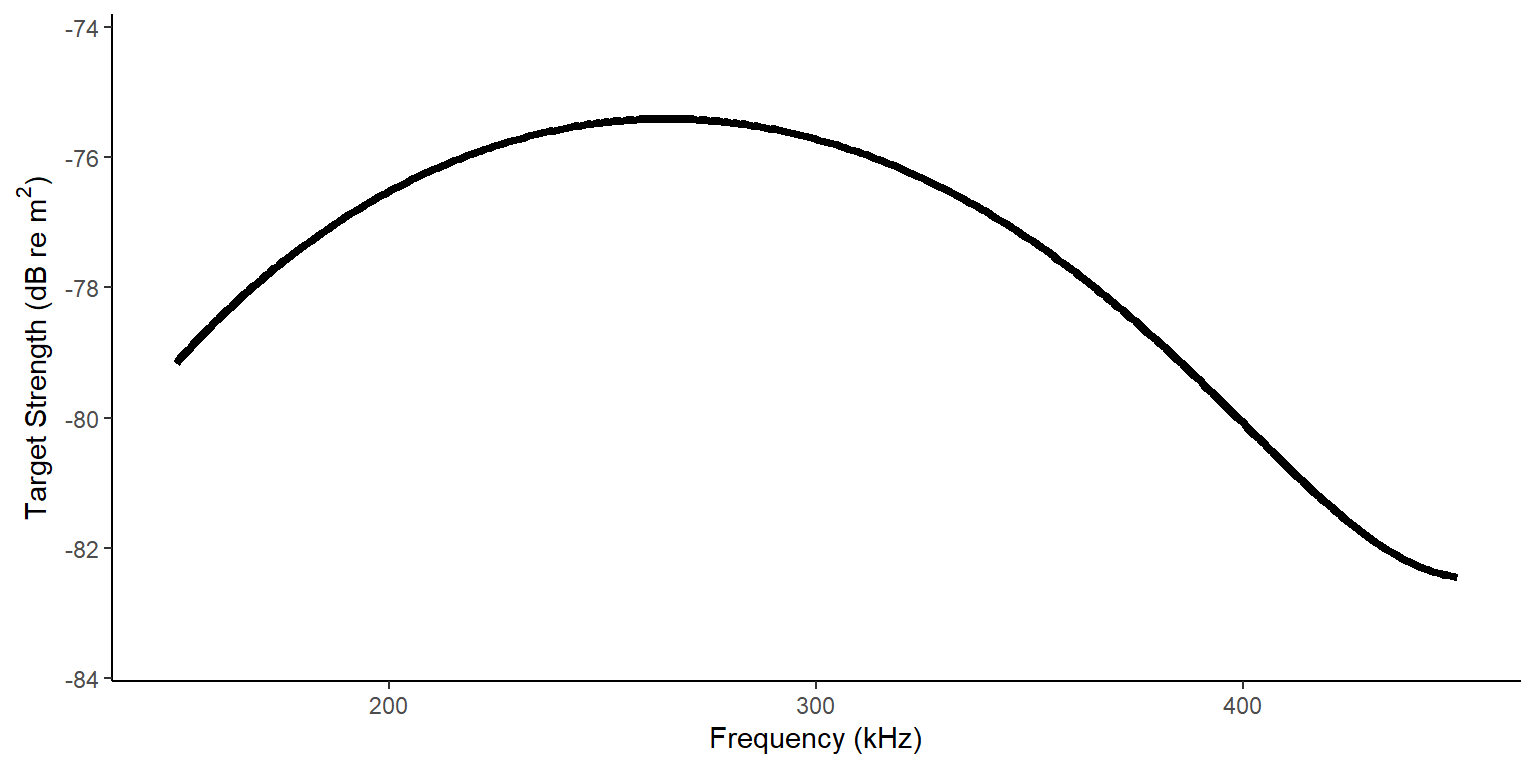
\includegraphics{sim_Muriel_files/figure-latex/unnamed-chunk-1-1.png}

To have a look at the overall distribution, we can also look at 2D
density plots:

\begin{Shaded}
\begin{Highlighting}[]
\NormalTok{pL <-}\StringTok{ }\ControlFlowTok{function}\NormalTok{(sim, title)\{}
  \KeywordTok{ggplot}\NormalTok{(}\DataTypeTok{data=}\NormalTok{sim, }\KeywordTok{aes}\NormalTok{(}\DataTypeTok{x=}\NormalTok{freq, }\DataTypeTok{y=}\NormalTok{TS))}\OperatorTok{+}
\StringTok{    }\KeywordTok{geom_density2d_filled}\NormalTok{()}\OperatorTok{+}
\StringTok{    }\CommentTok{#facet_wrap(.~spec, scales='free')+}
\StringTok{    }\KeywordTok{scale_x_continuous}\NormalTok{(}\DataTypeTok{expand=}\KeywordTok{c}\NormalTok{(}\DecValTok{0}\NormalTok{,}\DecValTok{0}\NormalTok{))}\OperatorTok{+}
\StringTok{    }\KeywordTok{scale_y_continuous}\NormalTok{(}\DataTypeTok{expand=}\KeywordTok{c}\NormalTok{(}\DecValTok{0}\NormalTok{,}\DecValTok{0}\NormalTok{))}\OperatorTok{+}
\StringTok{    }\KeywordTok{ggtitle}\NormalTok{(title)}\OperatorTok{+}
\StringTok{    }\KeywordTok{theme_classic}\NormalTok{()}
\NormalTok{\}}


\NormalTok{sim_tmp <-}\StringTok{ }\NormalTok{sim }\OperatorTok\StringTok{ }
\StringTok{  }\KeywordTok{group_by}\NormalTok{(spec) }\OperatorTok\StringTok{ }
\StringTok{  }\KeywordTok{nest}\NormalTok{() }\OperatorTok\StringTok{ }
\StringTok{  }\KeywordTok{mutate}\NormalTok{(}\DataTypeTok{plots =} \KeywordTok{map2}\NormalTok{(data, spec, pL))}
\NormalTok{pL =}\StringTok{ }\NormalTok{gridExtra}\OperatorTok{::}\KeywordTok{grid.arrange}\NormalTok{(}\DataTypeTok{grobs =}\NormalTok{ sim_tmp}\OperatorTok{$}\NormalTok{plots)}
\end{Highlighting}
\end{Shaded}

\includegraphics{sim_Muriel_files/figure-latex/unnamed-chunk-2-1.png}

\end{document}
